\section{Вычислительные эксперименты}
Используемые обозначения: \\
all\_speakers = дикторы speaker1, speaker2, speaker3, speaker4, speaker5, speaker6; \\
all\_male\_speakers = дикторы speaker1, speaker2, speaker3, speaker4, speaker5.
\subsection{Описание экспериментов}
Для каждого из двух типов нейронных сетей, многослойного персептрона и свёрточной сети, проводятся три эксперимента:
\begin{enumerate}[leftmargin=2cm]
	\item нейронная сеть обучается на первом дикторе с мужским голосом, тестирование производится сначала на каждом дикторе, а потом на всех вместе;
	\item нейронная сеть обучается на всех дикторах с мужским голосом, тестирование производится сначала на каждом дикторе, а потом на всех вместе;
	\item нейронная сеть обучается на всех дикторах, тестирование производится сначала на каждом дикторе, а потом на всех вместе.
\end{enumerate}

Обучение каждого из двух типов нейронных сетей производится со следующими параметрами:
\begin{itemize}[leftmargin=2cm]
	\item после каждой эпохи тренировочные данные перемешиваются;
	\item 15\% тренировочных данных в каждой эпохе - валидационные;
	\item метрика для оценки эффективности - точность (в библиотеке Keras называется accuracy);
	\item функция потерь - категориальная кросс-энтропия (в библиотеке Keras называется categorical\_crossentropy);
	\item алгоритм оптимизации - Adam;
	\item количество эпох обучения сети - 50;
	\item если в течение 20 эпох значение функции потерь на валидационных данных не уменьшается, то происходит ранняя остановка обучения сети.
\end{itemize}

В случае обучения на all\_speakers, помимо тестирования строится матрица путаницы (confusion matrix) для каждого из четырёх пороговых значений: 0.5, 0.6, 0.7, 0.8. Анализ матриц путаницы лежит за рамками данной работы. Используя его, можно подобрать оптимальное пороговое значение для более удобного использования интерфейса распознавания речевых команд уже при его внедрении в программное обеспечение медиаплеера. 

Смысл порогового значения следующий: eсли максимальный элемент в выходном тензоре нейронной сети ниже порогового значения, то команда определяется как нераспознанная (далее в матрицах путаницы используется сокращение <<нераспозн.>>). В этом случае интерфейс медиаплеера просит повторить команду ещё раз. Если максимальный элемент в выходном тензоре нейронной сети выше или равен пороговому значению, то команда распознаётся как соответствующая индексу этого максимального элемента. 

\newpage
\subsection{Результаты экспериментов}
Графики обучения многослойного персептрона приведены на рисунках \ref{fig:mlp_speaker1_train_graphs}, \ref{fig:mlp_all_male_speakers_train_graphs}, \ref{fig:mlp_all_speakers_train_graphs}.

\begin{figure}[H]
	\[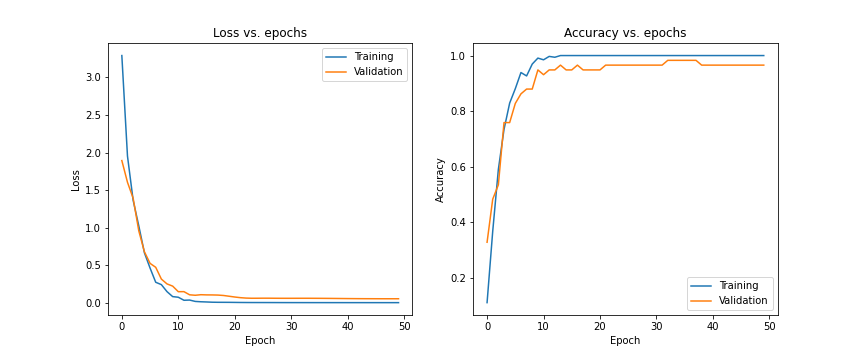
\includegraphics[scale=0.4]{mlp_speaker1_train_graphs.png}\]
	\caption{Графики функций потерь и точности многослойного персептрона в течение обучения на speaker1}
	\label{fig:mlp_speaker1_train_graphs}
\end{figure}

\begin{figure}[H]
	\[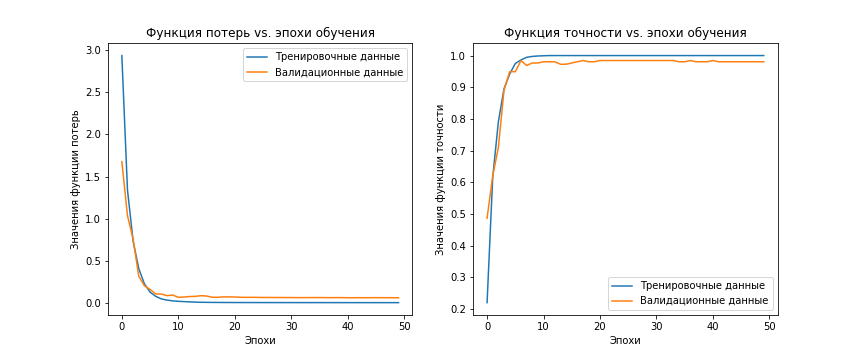
\includegraphics[scale=0.4]{mlp_all_male_speakers_train_graphs.png}\]
	\caption{Графики функций потерь и точности многослойного персептрона в течение обучения на all\_male\_speakers}
	\label{fig:mlp_all_male_speakers_train_graphs}
\end{figure}

\begin{figure}[H]
	\[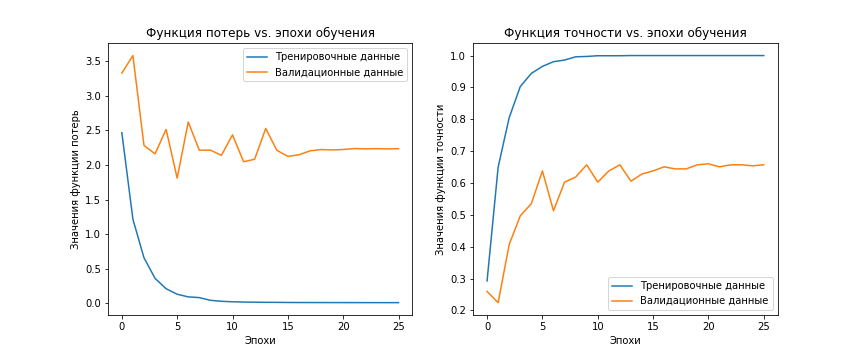
\includegraphics[scale=0.4]{mlp_all_speakers_train_graphs.png}\]
	\caption{Графики функций потерь и точности многослойного персептрона в течение обучения на all\_speakers}
	\label{fig:mlp_all_speakers_train_graphs}
\end{figure}


Графики обучения свёрточной сети приведены на рисунках \ref{fig:cnn_speaker1_train_graphs}, \ref{fig:cnn_all_male_speakers_train_graphs}, \ref{fig:cnn_all_speakers_train_graphs}.

\begin{figure}[H]
	\[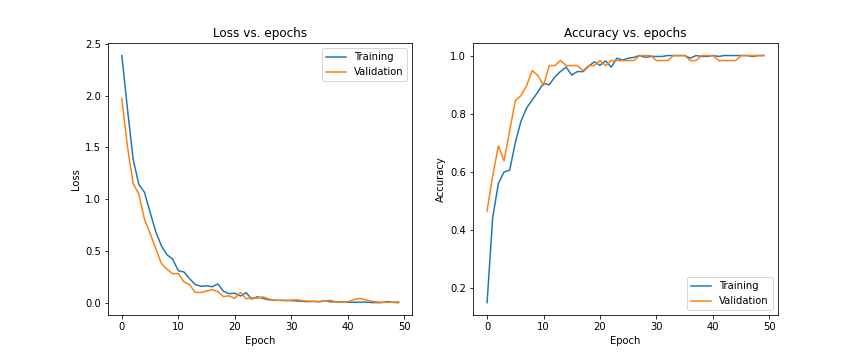
\includegraphics[scale=0.4]{cnn_speaker1_train_graphs.png}\]
	\caption{Графики функций потерь и точности свёрточной сети в течение обучения на speaker1}
	\label{fig:cnn_speaker1_train_graphs}
\end{figure}

\begin{figure}[H]
	\[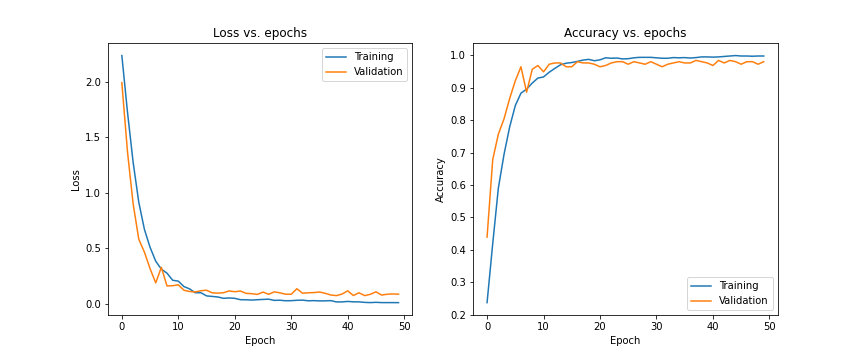
\includegraphics[scale=0.4]{cnn_all_male_speakers_train_graphs.png}\]
	\caption{Графики функций потерь и точности свёрточной сети в течение обучения на all\_male\_speakers}
	\label{fig:cnn_all_male_speakers_train_graphs}
\end{figure}

\begin{figure}[H]
	\[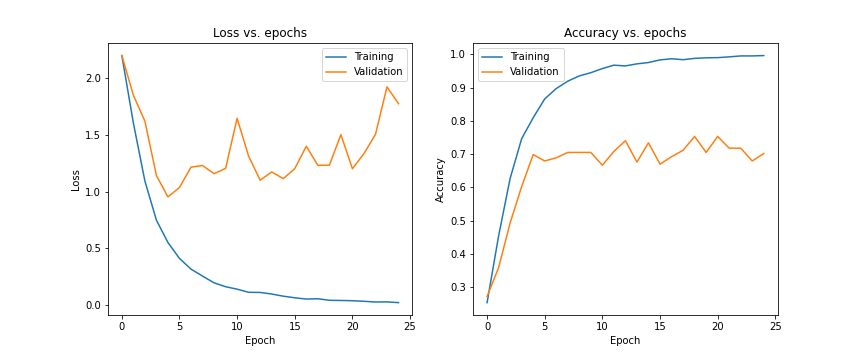
\includegraphics[scale=0.4]{cnn_all_speakers_train_graphs.png}\]
	\caption{Графики функций потерь и точности свёрточной сети в течение обучения на all\_speakers}
	\label{fig:cnn_all_speakers_train_graphs}
\end{figure}

\newpage
Матрицы путаницы для многослойного персептрона при обучении на all\_speakers представлены на рисунке \ref{fig:mlp_cm_all_speakers}.

\begin{figure}[H]
	\[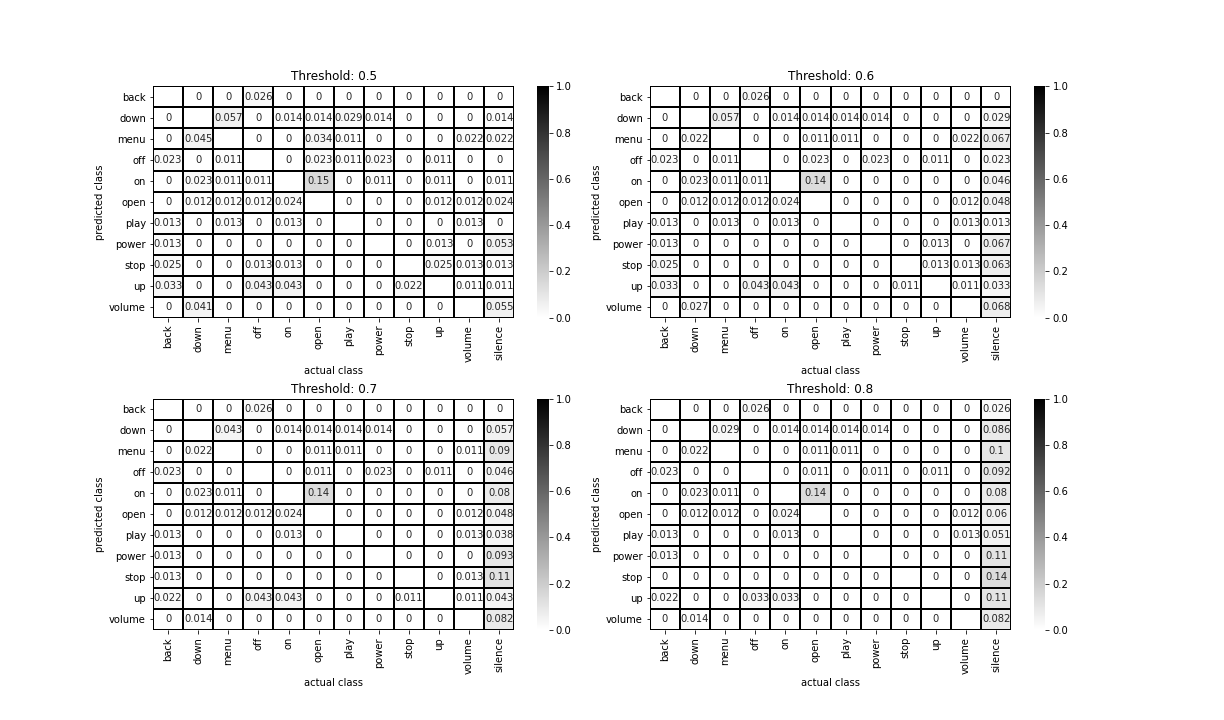
\includegraphics[scale=0.4]{mlp_cm_all_speakers.png}\]
	\caption{Матрицы путаниц для многослойного персептрона при обучении на all\_speakers}
	\label{fig:mlp_cm_all_speakers}
\end{figure}

\newpage
Матрицы путаницы для свёрточной сети при обучении на all\_speakers представлены на рисунке \ref{fig:cnn_cm_all_speakers}.

\begin{figure}[H]
	\[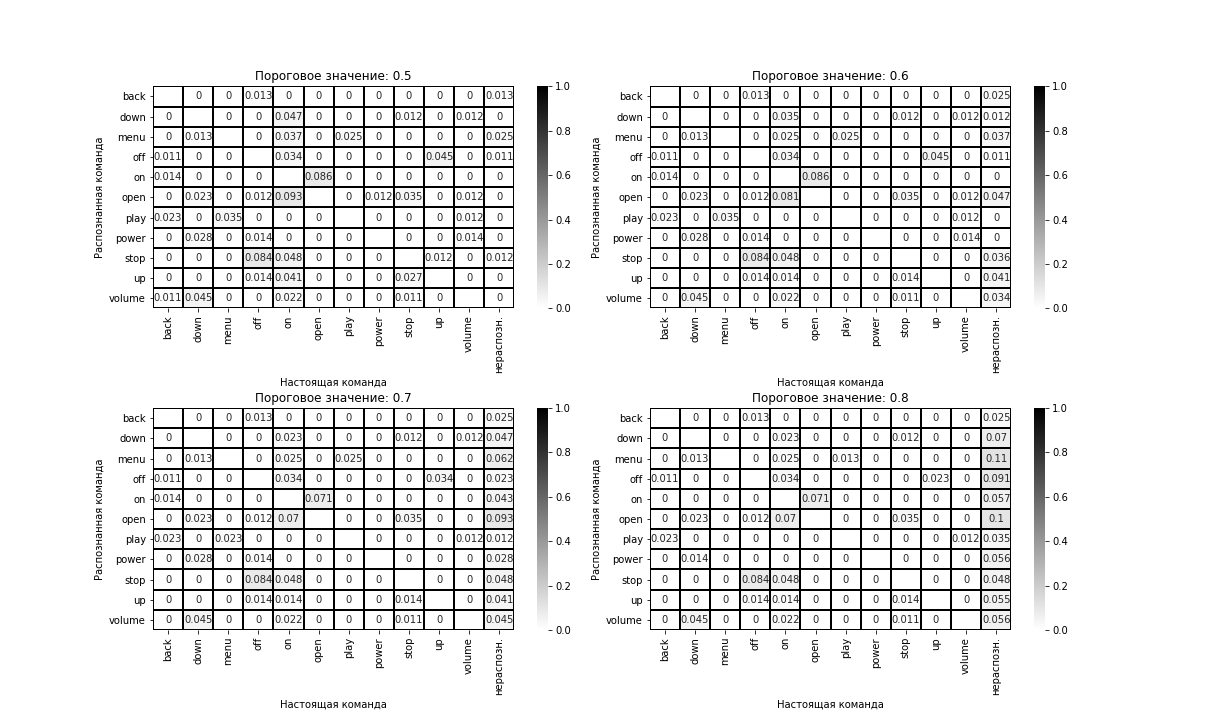
\includegraphics[scale=0.4]{cnn_cm_all_speakers.png}\]
	\caption{Матрицы путаницы для свёрточной сети при обучении на all\_speakers}
	\label{fig:cnn_cm_all_speakers}
\end{figure}

\newpage
Результаты тестирования представлены в таблице \ref{table:test_summary}. Используемые обозначения: train\_data - тренировочные данные, test\_data - тестовые данные, cnn\_loss - значения функции потерь для свёрточной сети, mlp\_loss - значения функции потерь для многослойного персептрона, cnn\_accuracy - значения функции точности для свёрточной сети, mlp\_accuracy - значения функции точности для многослойного персептрона.

\begin{table}[H]
\small
\centering
\csvautotabular[respect underscore=true]{csv/test_summary.csv}
\caption{Результаты тестирования}
\label{table:test_summary}
\end{table}